\documentclass{article}
\usepackage{amsmath}
\usepackage{amssymb}
\usepackage{ctex}
\usepackage[margin=2cm]{geometry} % 设置较窄的边距使文档宽一些
\usepackage{multirow} % 支持表格中的多行单元格
\usepackage{graphicx} % 用于插入图片
\usepackage{subcaption} % 支持子标题
\usepackage{float} % 支持 [H] 浮动体选项
\title{\heiti\zihao{2}实验三\quad 三相交流电路电压、电流的测量 }
\author{\songti  孙振川  PB23081463 \\
课程号  ME2011.04 }
\date{2025.5.26}
\begin{document}
    \maketitle
\begin{abstract}
    
    通过平衡负载和非平衡负载实验,掌握三相负载作星形联接、三角形联接的方法,验证线、相电压及线、相电流之间的关系,以及中性线的作用
    
    \noindent{\textbf{关键词:} 三相负载;星形联接;三角形联接;线电压;相电压;线电流;相电流;中性线}
\end{abstract}
\section{实验目的}
\begin{enumerate}
    \item 掌握三相负载作星形联接、三角形联接的方法,验证这两种接法下线、相电压及线、相电流之间的关系。 
    \item 充分理解三相四线供电系统中中线的作用。
\end{enumerate}

\section{实验原理}
1.三相负载可接成星形(又称"Y"接)或三角形(又称"$\triangle$"接)。当三相对称负载作星形联接时,线电压 $U_1$ 是相电压 $U_p$ 的 $\sqrt{3}$ 倍。线电流 $I_1$ 等于相电流 $I_p$ ,即

$$
\mathrm{U}_{\mathrm{l}}=\sqrt{3} U_P, \quad \mathrm{I}_1=\mathrm{I}_{\mathrm{p}}
$$


在这种情况下,流过中线的电流 $\mathrm{I} 0=0$ ,所以可以省去中线。由三相三线制电源供电,无中线的星形联接称为 Y 接法。

当对称三相负载作 $\triangle$ 形联接时,有 $\mathrm{I}_1=\sqrt{3} \mathrm{I}_{\mathrm{p}}, \quad \mathrm{U}_1=\mathrm{U}_{\mathrm{p}}$ 。
2.不对称三相负载作星形联接时,必须采用三相四线制接法,即 $Y_o$ 接法。而且中线必须牢固联接,以保证三相不对称负载的每相电压维持对称不变。

倘若中线断开,会导致三相负载电压的不对称,致使负载轻的那一相的相电压过高,使负载遭受损坏;负载重的一相相电压又过低,使负载不能正常工作。尤其是对于三相照明负载,无条件地一律采用 $\mathrm{Y}_0$ 接法。

3.当不对称负载作 $\triangle$ 接时, $\mathrm{I}_1 \neq \sqrt{3} \mathrm{I}_p$ ,但只要电源的线电压 $\mathrm{U}_1$ 对称,加在三相负载上的电压仍是对称的,对各相负载工作没有影响。

\section{实验器材}
\label{sec:equipment}
    \begin{enumerate}
        \item 交流电压表  0~500V 
        \item 交流电流表 0~5A 
        \item 万用表
        \item 三相自耦调压器 
        \item 三相灯组负载 220V,25W 白炽灯 
        \item 电流插座
    \end{enumerate} 

\section{实验内容}
\subsection{三相负载星形联接(三相四线制供电) }
按图 1 线路组接实验电路。即三相灯组负载经三相自耦调压器接通三相对称电源。将三相

调压器的旋柄置于输出为 0 V 的位置(即逆时针旋到底)。经指导教师检查合格后,方可开启实验台电源,
然后调节调压器的输出,使输出的三相线电压为 220 V,并按下述内容完成各项实验,
分别测量三相负载的线电压、相电压、线电流、相电流、中线电流、电源与负载中点间的电压。
将所测得的数据记入表 1 中,并观察各相灯组亮暗的变化程度,特别要注意观察中线的作用。
\begin{figure}[H]
    \centering
    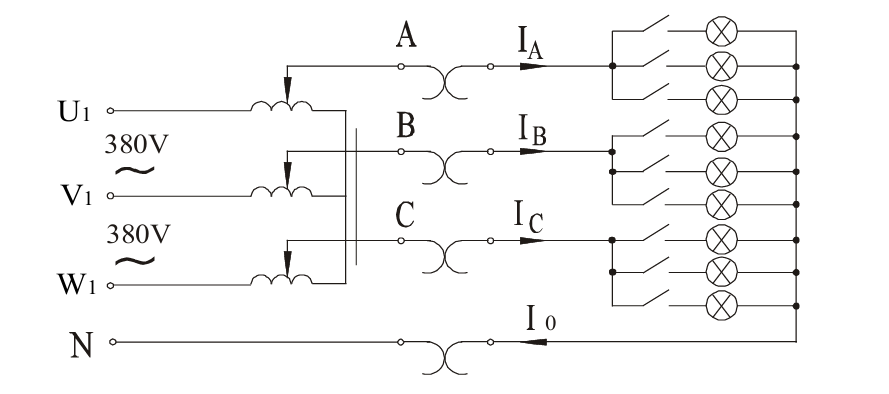
\includegraphics[width=0.8\textwidth]{img1.png}
    \caption{三相负载星形联接实验电路图}
    \label{fig:star_connection_circuit}
\end{figure}

\begin{figure}[H]
    \centering
    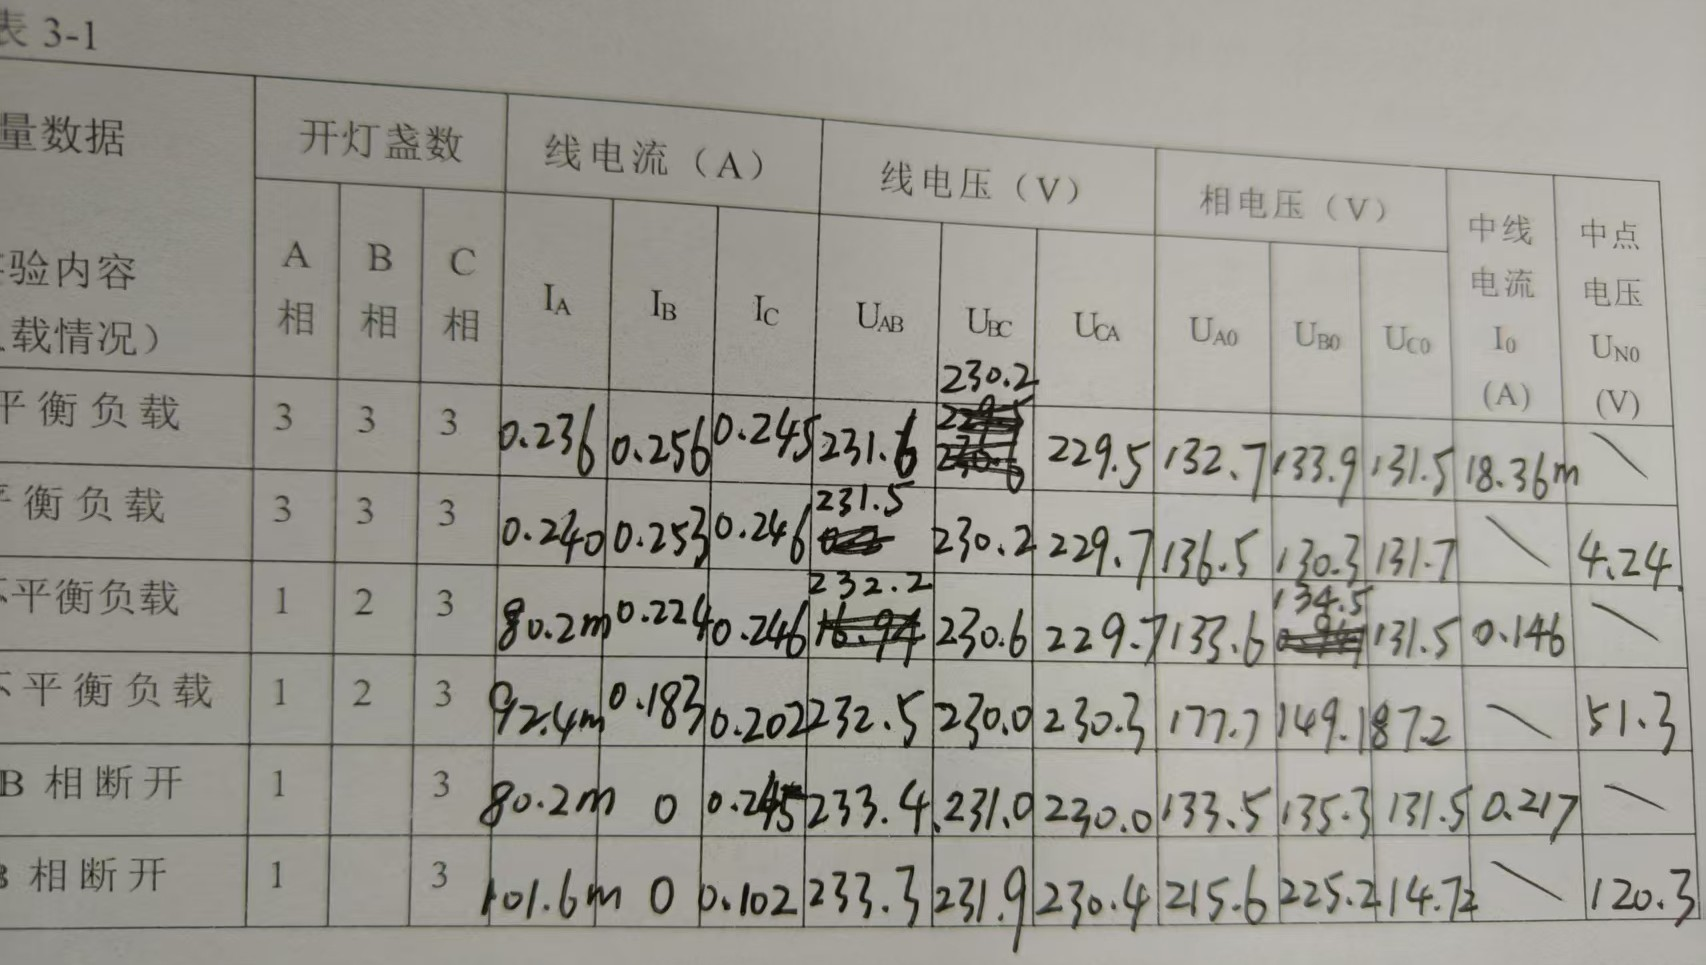
\includegraphics[width=0.8\textwidth]{table1.jpg}
\end{figure}

\subsection{ 负载三角形联接(三相三线制供电)}
按图 2 改接线路,经指导教师检查合格后接通三相电源,并调节调压器,使其输出线电压为 220 V,并按表 3-2 的内容进行测试。

\begin{figure}[H]
    \centering
    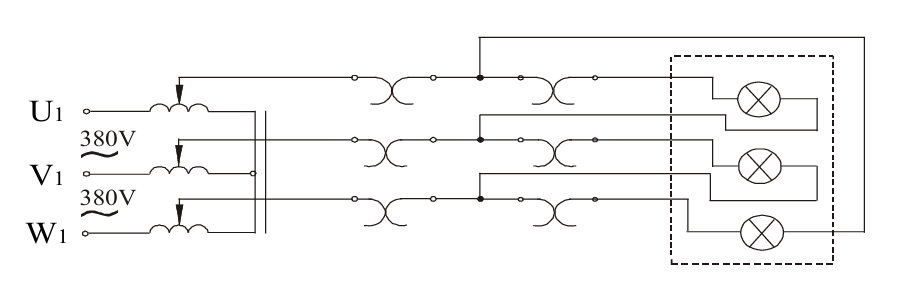
\includegraphics[width=0.8\textwidth]{img2.png}
    \caption{负载三角形联接实验电路图}
\end{figure}

\begin{figure}[H]
    \centering
    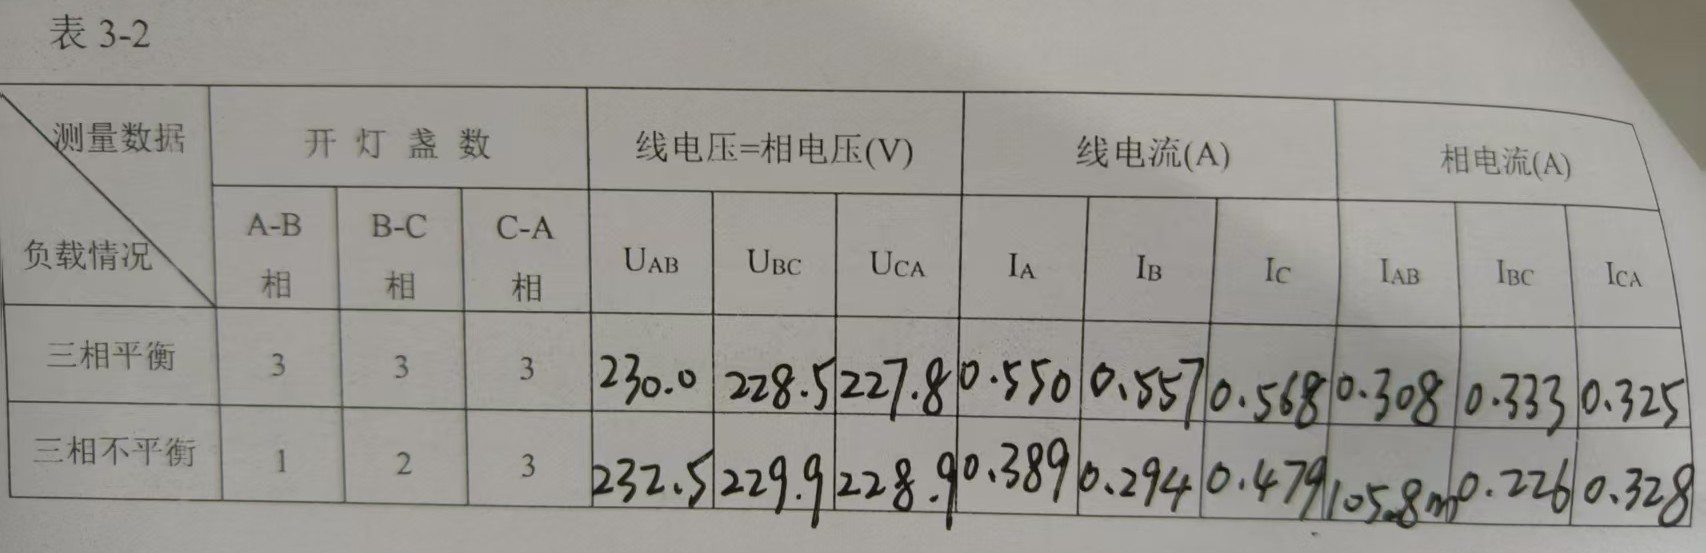
\includegraphics[width=0.8\textwidth]{table2.jpg}
\end{figure}

\section{实验数据处理 }
\subsection{ 验证对称三相电路中的$ \sqrt{3} $关系}
\begin{figure}[H]
    \centering
    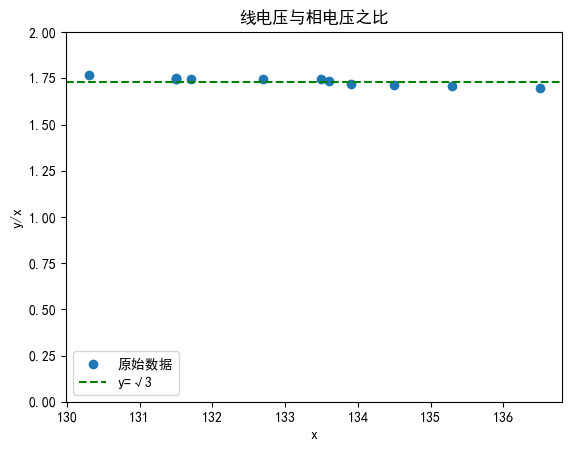
\includegraphics[width=0.5\textwidth]{output1.png}
    \caption{验证对称三相电路中的$ \sqrt{3} $关系}
\end{figure}
\subsection{三相四线供电系统中中线的作用}
三相四线制中线的作用是流过三相负载的不平衡电流,来保持中性点的零点位,使负载电压保持不变。如果中线断了,不平衡的三相负载使得中性点转移,使负载最少的那一相电压最高负载因过电压损坏,而负载多的那一相电压过低无法工作。
中线流过三相负载的不平衡电流,来保持中性点的零点位,使负载电压保持不变



\subsection{不对称三角形联接的负载,能否正常工作?实验是否能证明这一点? }
能,不对称三相负载的三角形连接时,线电压等于相电压,线电流等于 $\sqrt{3}$ 倍的相电流。只要线电压对称,加在三相负载上的电压仍是对称的,对各相负载工作没影响。即使某一相负载开路或短路,其他两相负载仍可正常工作。只要线电压等于负载额定电压就可以正常工作,不需要中线的帮助。

\subsection{根据不对称负载三角形联接时的相电流值作相量图,并求出线电流值,然后与实验测得的线电流作比较,分析之。}
$$
\begin{aligned}
& I_a=I_{ab}-I_{ca} \\
&I_b=I_{bc}-I_{ab}\\
& I_c=I_{ca}-I_{bc} 
\end{aligned}
$$

\begin{figure}[H]
    \centering
    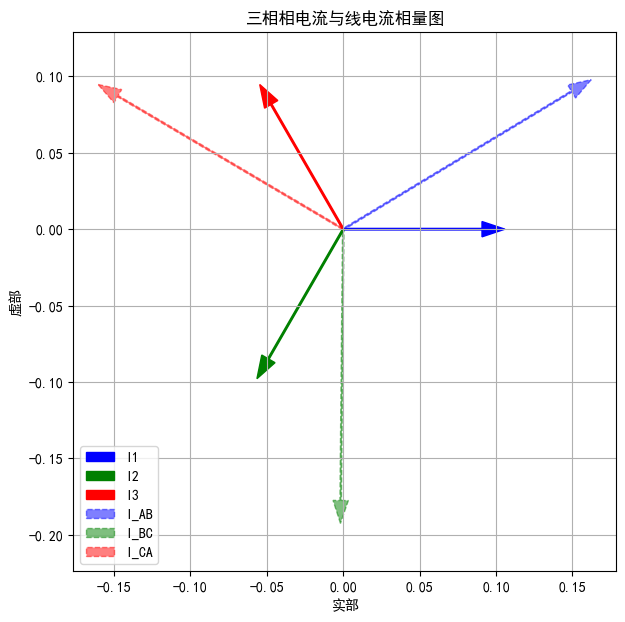
\includegraphics[width=0.5\textwidth]{output2.png}
    \caption{不对称负载三角形联接的相量图}
\end{figure}



理论线电流(A): [0.293 0.482 0.391]

实验线电流(A): [0.294 0.479 0.389]

理论 - 实验差值: [-0.001  0.003  0.002]



\section{预习思考题 }
\subsection{ 三相负载根据什么条件作星形或三角形连接?}

三相负载星形或三角形连接,是根据绕组(如电动机)或用电器的额定电压连接的。或者说三相负载根据负载设计的额度电压和实际的电源电压决定星形或三角形连接。

由对称三相供电系统对三相星形连接负载供电时,若三相负载相等,即 ZA=ZB=ZC=Z,则每相负载上所加的电压是三相系统线电压的 $1 / \sqrt{3}$ 。所以每相额定电压为 220 伏的三相感应电动机,用线电压为 380 伏的三相电源供电时,必须接成星形。

一台每相额定电压为 380 伏的三相感应电动机,只有连接成三角形才能接到线电压为 380 伏的三相电源使用。三角形连接的负载只要三相电源是对称的,三相负载电压也一定是对称的,各相负载电流在电源电压一定时也只与该相的阻抗有关。

例如:
1、负载额定电压 220 V,电源额定电压 380 V,就接成星形连接,这时负载获得 220 V 电压。
2、负载额定电压 220 V,电源额定电压 220 V,就接成三角形连接,这时负载获得 220 V 电压。
3、负载额定电压 380 V,电源额定电压 380 V,就接成三角形连接,这时负载获得 380 V 电压。


\subsection{ 复习三相交流电路有关内容,试分析三相星形联接不对称负载在无中线情况下,当某相
负载开路或短路时会出现什么情况?如果接上中线,情况又如何?}

1、当某相负载开路时,就相当于另外两组串联在 380 V 电压下使用,那么电阻大的那组,分得的电压高,如超过其额定电压 Q 就会烧毁。

2、如某相负载短路,那么另外两组都处于 380 V 电压下,都将烧毁。

3、如接上中线,可正常使用,中线有电流。。

\subsection{本次实验中为什么要通过三相调压器将 380V 的市电线电压降为 220V 的线电压使用? }

为了实验设备(负载)不被损坏


\section{总结感悟 }
本次实验通过对三相负载的星形和三角形连接的实验,深入理解了三相交流电路的基本原理和应用。通过测量线电压、相电压、线电流、相电流等参数,验证了三相电路中线、相电压及线、相电流之间的关系。同时,通过观察中性线的作用,认识到在不对称负载情况下,中性线的重要性。
在实验中,星形连接和三角形连接的负载表现出不同的电气特性,特别是在对称和不对称负载情况下的电流分布和电压关系。通过对比理论计算和实验数据,发现实际测量结果与理论值存在一定的误差,这可能是由于实验设备的精度限制以及实际元件的非理想特性所致。


\section{参考文献}
\begin{enumerate}
    \item 电子电路实验指导书
    \item 电子电路基础
    \item 电路原理
    \item 电路分析
\end{enumerate} 

\end{document}

